\begin{figure}[!]
    \centering
    \captionlistentry{(a) Level Scheme of $^{156}$Gd. The gamma ray of the $2^+_{gs}\rightarrow 0^+_{gs}$ (89 keV) transition in the ground state was gated on. It was then compared with the gated spectrum from the gamma ray of the $4^+_{gs}\rightarrow 2^+_{gs}$ (199 keV) transition in the ground state. Peaks only appearing in the first gate were assumed to go into the $2^+_{gs}$ state, and assignments were made. Due to the low energy of the $2^+_{gs}\rightarrow 0^+_{gs}$ transition, the efficiency was lower, and it is likely that transitions into the $2^+_{gs}$ state were missed. The levels are organized by band. The lower levels of the band, unseen by gamma rays in this gate, are in blue. (b) Gamma spectrum gated on 89 keV, corresponding to the $2^+_{gs}\rightarrow 0^+_{gs}$ transition. Several transitions are marked according to the level scheme.}
    \label{fig:156_2to0}
    \begin{subfigure}{\textwidth}
    \caption{\centering \fontsize{10pt}{12pt}Level Scheme of $^{156}$Gd. The gamma ray of the $2^+_{gs}\rightarrow 0^+_{gs}$ (89 keV) transition in the ground state was gated on. It was then compared with the gated spectrum from the gamma ray of the $4^+_{gs}\rightarrow 2^+_{gs}$ (199 keV) transition in the ground state. Peaks only appearing in the first gate were assumed to go into the $2^+_{gs}$ state, and assignments were made. Due to the low energy of the $2^+_{gs}\rightarrow 0^+_{gs}$ transition, the efficiency was lower, and it is likely that transitions into the $2^+_{gs}$ state were missed. The levels are organized by band. The lower levels of the band, unseen by gamma rays in this gate, are in blue. (b) Gamma spectrum gated on 89 keV, corresponding to the $2^+_{gs}\rightarrow 0^+_{gs}$ transition. Several transitions are marked according to the level scheme.}
    \end{subfigure}
\end{figure}
\clearpage
\begin{figure}
    \ContinuedFloat
    \begin{subfigure}{\textwidth}
    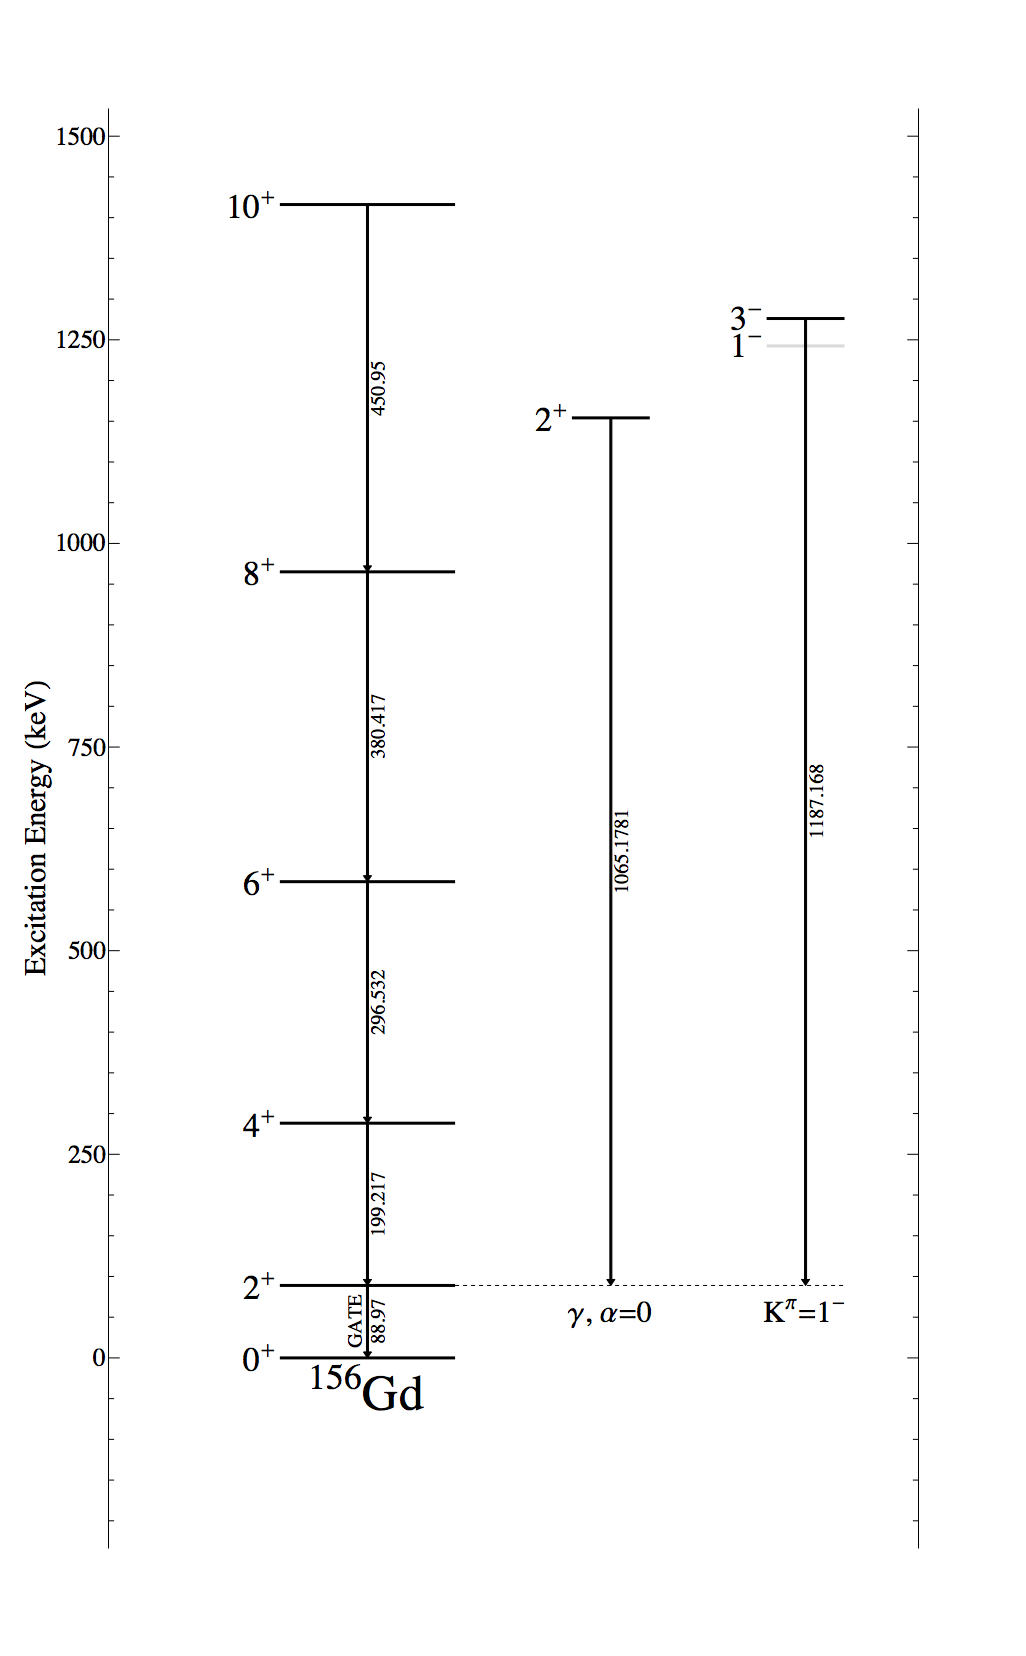
\includegraphics[scale=0.4]{156GdTablesAndFigs/156Gd_2to0.eps}
    \caption*{(a)}
    \label{fig:156_2to0level}
    \end{subfigure}
    \end{figure}
    \begin{figure}
    \ContinuedFloat
    \begin{subfigure}{\textwidth}
    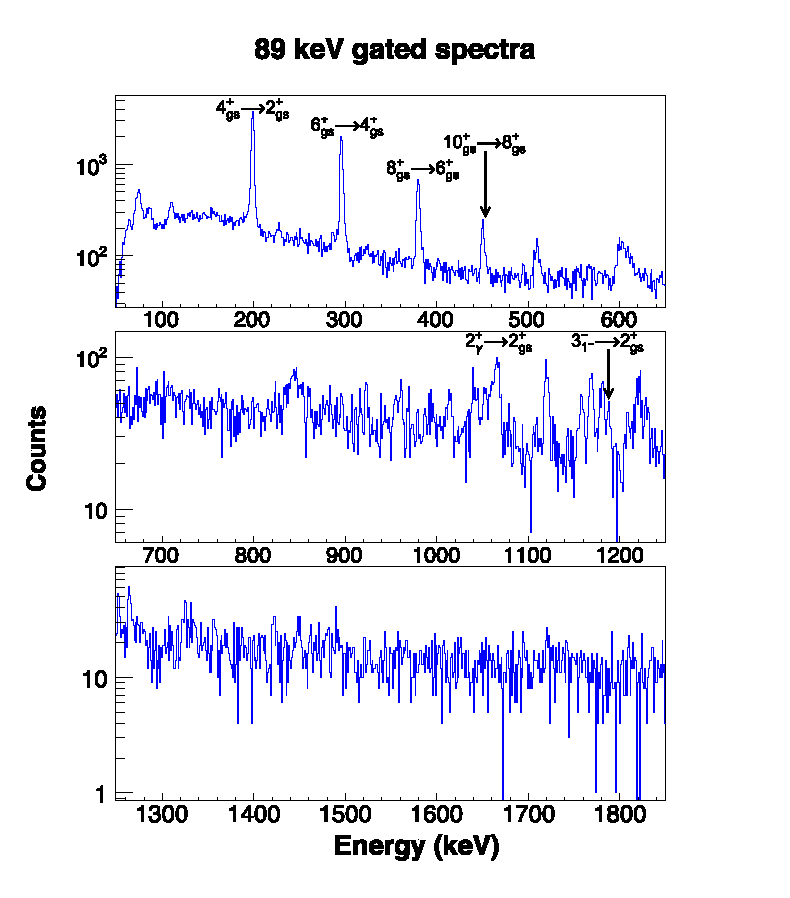
\includegraphics[scale=1.3]{156GdTablesAndFigs/89_gamma.eps}
    \caption*{(b)}
    \label{fig:156_2to0spec}
    \end{subfigure}
\end{figure}